\section{Proposed Technique}

\subsection{Approach Overview}
Agrasandhani is an end-to-end MQTT pipeline that treats sensor updates as a stream to be cleaned, summarized, and delivered with stable dashboard semantics. The system has four components. (1) A Python/asyncio \emph{sensor simulator} generates a mixed workload (slowly-changing and spiky sensors) and publishes JSON messages of the form \texttt{\{sensor\_id, msg\_id, ts\_sent, value, type\}} to an MQTT topic (e.g., \texttt{sensors/raw}), allowing unambiguous measurement of duplicates and latency. (2) A standard \emph{MQTT broker} (Mosquitto) relays messages using MQTT QoS 0 and QoS 1; QoS 1 provides ``at least once'' delivery and may introduce duplicates via retransmission, which motivates message-level deduplication in the gateway \cite{mqtt311}. (3) The \emph{smart gateway} subscribes to \texttt{sensors/raw} and emits aggregated updates to \texttt{gateway/agg} using an ablation ladder of policies: V0 forwards every message; V1 performs hybrid batching (flush every $T$ ms or when $K$ messages accumulate); V2 adds two-stage deduplication (drop exact duplicates by \texttt{msg\_id} and compact each batch to the latest update per sensor); V3 adapts the publish rate by adjusting $T$ based on observed publish health (send time/backlog), using a simple control law where if backlog $> B$ or publish time EMA $> P$ for $M$ consecutive flushes then $T \leftarrow \min(\alpha T, T_{\max})$, else $T \leftarrow \max(T/\alpha, T_{\min})$; and V4 combines V3 with last-known-good semantics by ensuring the dashboard can hold prior values and expose freshness (age) with a TTL. (4) A lightweight \emph{dashboard backend} subscribes to \texttt{gateway/agg} and pushes updates to a browser UI via WebSockets, where the UI displays the latest value per sensor along with an explicit \texttt{age} indicator and TTL-based staleness marking. To study robustness under degraded connectivity, we apply deterministic network impairments primarily on the gateway-to-dashboard path (bandwidth caps, loss, delay, jitter, and short outages) using Linux traffic control; \texttt{tc netem} supports controlled delay/loss/jitter/duplication for repeatable experiments.

\begin{figure}[t]
  \centering
  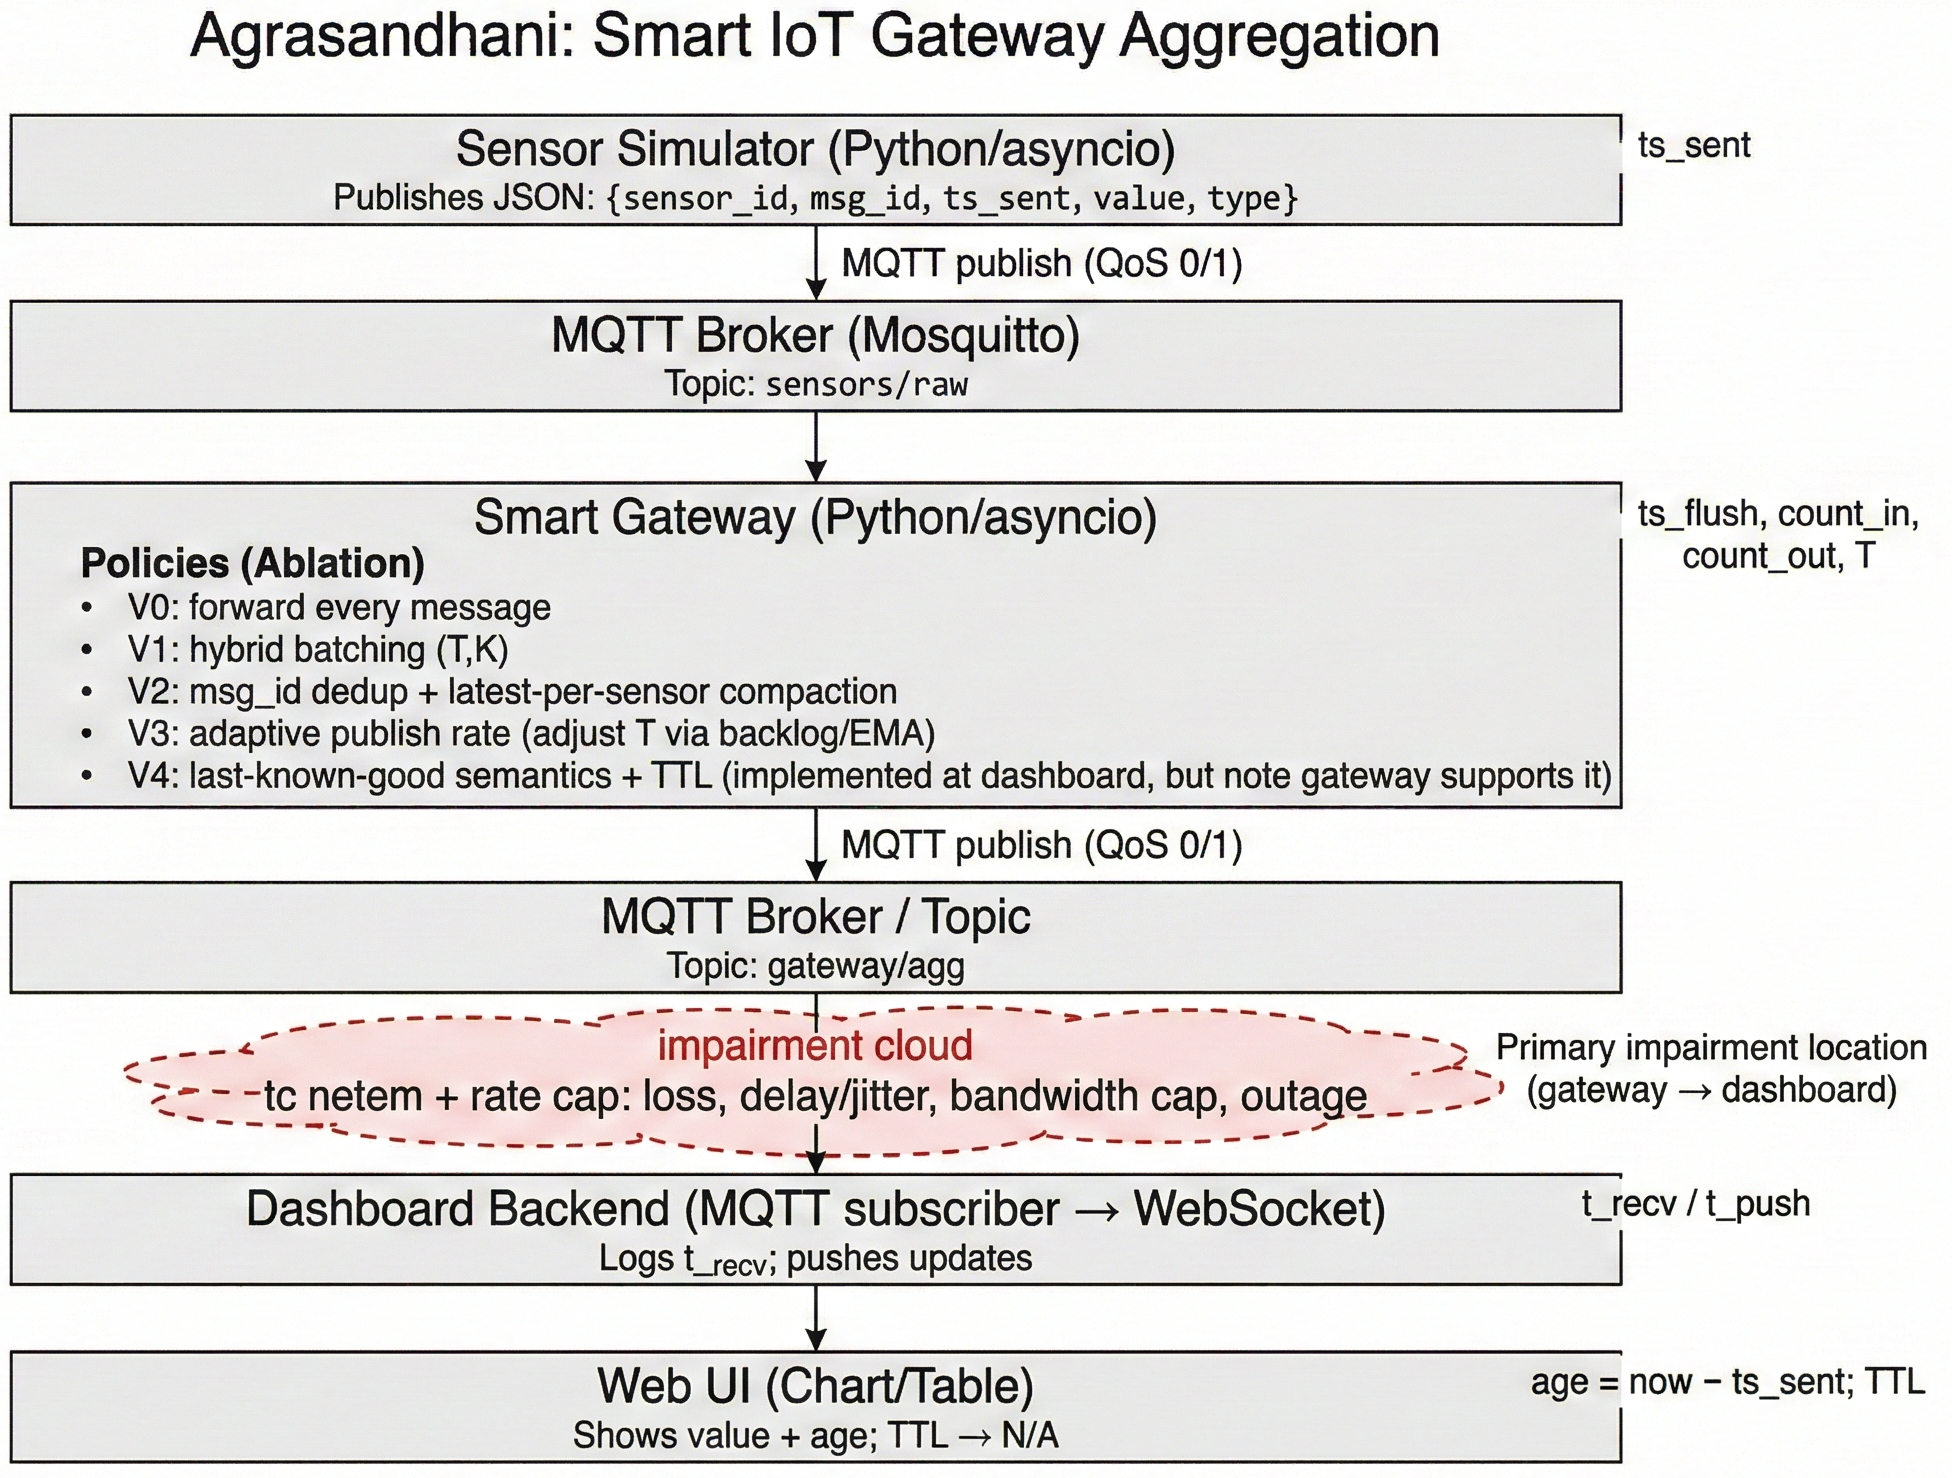
\includegraphics[width=\linewidth,height=\textheight,keepaspectratio]{Sections/approach-cs537.png}
  \caption{Agrasandhani end-to-end pipeline.}
  \label{fig:architecture}
\end{figure}

% \subsection{Approach Details}
% Describe the details of each component in this subsection
